\documentclass[a4paper,10pt]{article}
% This line indicates the type of the document betwin {}: here it is a scientific article.
% Options betwin [] are not mandatory, but precise here:
% - a4paper: printing paper format
% - 10pt: size of the characters

\usepackage{graphicx}
% This package allows to include images
\usepackage{titling}
% This package allows to have a subtitle 
\usepackage{listings}
\usepackage{float}
\usepackage{hyperref}
\usepackage{booktabs}
\usepackage{algorithm}
\usepackage{algpseudocode}

\usepackage[table,xcdraw]{xcolor}

% this package is used to write code samples.
\lstset{%
  basicstyle=\scriptsize\sffamily,%
  commentstyle=\footnotesize\ttfamily,%
  frameround=trBL,
  frame=single,
  breaklines=true,
  showstringspaces=false,
  numbers=left,
  numberstyle=\tiny,
  numbersep=10pt,
  keywordstyle=\bf
}
\newcommand{\subtitle}[1]{%
  \posttitle{%
    \par\end{center}
    \begin{center}\large#1\end{center}
    \vskip0.5em}%
}



%%%%%%%%%%%%%%%%%%%%%%%%%%%%%%%%%%%%%%%%%%%%%%%%%%%%
% Raport Headers:
%%%%%%%%%%%%%%%%%%%%%%%%%%%%%%%%%%%%%%%%%%%%%%%%%%%%
\title{Mathematics for Computer Science \\ Fair division of jewels}
\subtitle{Master MoSIG, Université Grenoble Alpes \& ENSIMAG}
\author{Ahmad Ghalawinji\\ \href{mailto:ahmad.ghalawinji@grenoble-inp.org}{\color{blue}ahmad.ghalawinji@grenoble-inp.org}}
\date{November 18, 2022}








\begin{document}
% Beginning serious stuff.


\maketitle

  {\hbox to0pt{\vbox{\baselineskip=10dd\hrule\hbox
to\hsize{\vrule\kern3pt\vbox{\kern3pt
\hbox{{\small I declare that this report is my own, original work. Without any group member.}}

\kern3pt
}\hfil%\kern3pt
\vrule
}\hrule}
}}
% Actually prints title / subtitle / authors and dat into the document


%%%%%%%%%%%%%%%%%%%%%%%%%%%%%%%%%%%%%%%%%%%%%%%%%%%%
% Abstract
%%%%%%%%%%%%%%%%%%%%%%%%%%%%%%%%%%%%%%%%%%%%%%%%%%%%




\begin{abstract}
The purpose of this report is to summarized the study about mathematical properties of a necklace splitting combinatorial problem. We can define the problem as follow, two thieves Alice and Bob meet after a robbery. They want to share the
loot (that is a necklace made of jewels) in a fair way. In this report we will use the following notations:
\begin{itemize}
    \item \texttt{n:} the number of jewels in the necklace.
    \item \texttt{k:} the number of jewels types.
    \item \texttt{cuts:} the number of needed cuts to divide the necklace fairly.
\end{itemize}
\end{abstract}


\section{Two types of jewels}
In this part we will prove that the problem of k = 2 types of jewels can be solved in at most 2 cuts.In order to do that we formalized the following assumptions: \begin{itemize}
    \item n : the number of jewels in the necklace, n is even.
    \item the jewels in the necklace are arranged randomly.
    \item k = 2, the number of jewels types.
\end{itemize}
We will start by a counter example, n = 12, k = 2. Figure \ref{1} showed the case where we can divide  the necklace on the middle and we will have the same number of each jewel types distributed fairly between Alice and Bob ( the two intervals after cutting the necklace ).


\begin{figure}[H]
  \centering
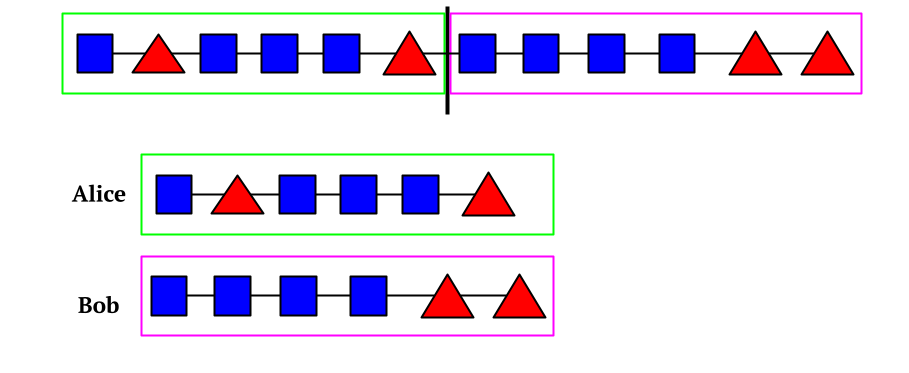
\includegraphics[scale=.35]{k=2 , cuts = 1.png}
\caption{n = 12, k = 2, cuts = 1}
\label{1}
\end{figure}















Figure \ref{2} illustrated the case where we need 2 cuts to divide the necklace.
\begin{figure}[H]
  \centering
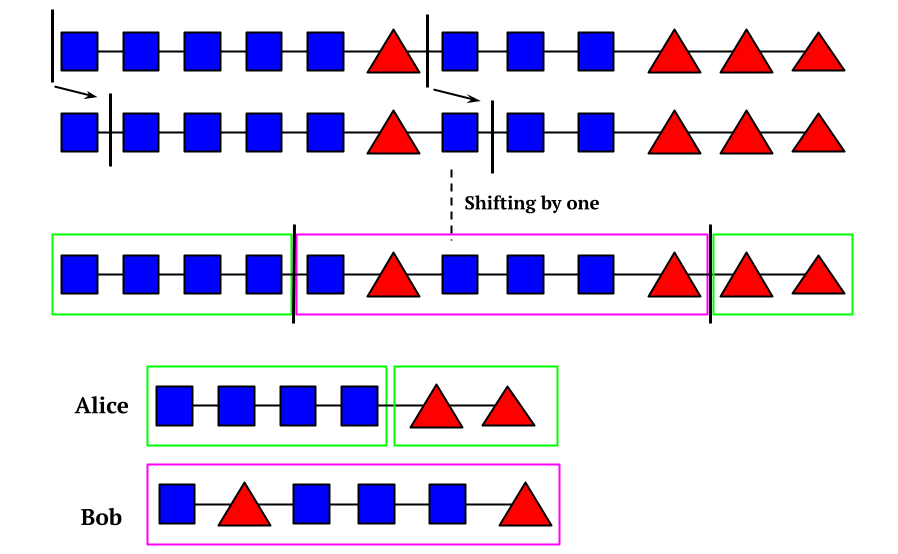
\includegraphics[scale=.35]{Copy of k=2 , generalize (2).png}
\caption{n = 12, k = 2, cuts = 2}
\label{2}
\end{figure}

In the previous example, we can recognized that two cuts are always enough for splitting the necklace. First we split the necklace into two half, if one half have two few diamonds that implies that the other half have too many. By shifting the interval one to the right the number of diamonds will change by one, therefore, we guarantee that at one point we will have the same number of diamonds in the two half. As a result, the number of rubies would be equal in the two half, since the total number of jewels is dividable by 2 and we just have two types. We could generalize the previous case according to the total number of jewels as shown in figure \ref{3}

\begin{figure}[H]
  \centering
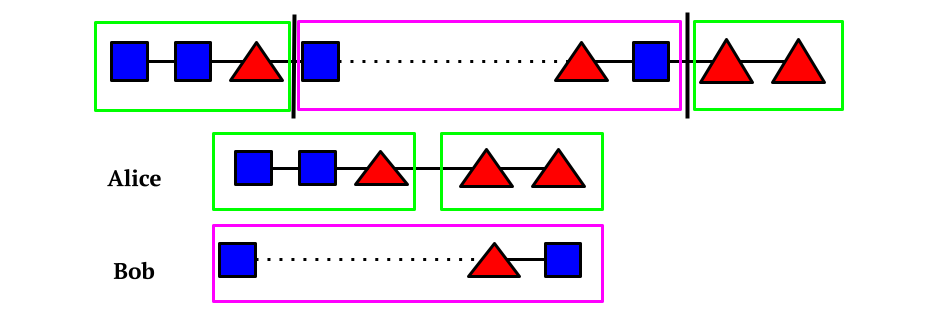
\includegraphics[scale=.35]{k = 2, cuts = 2.png}
\caption{k = 2, cuts = 2}
\label{3}
\end{figure}



\section{Three types of jewels}

In this part we will introduce a counter example to show that with 3-types of jewels two cuts will not be sufficient. We have the following configuration,as shown in figure \ref{4}
\begin{itemize}
    \item n = 12 (4 rubies, 6 diamonds, 2 sapphires)
    \item k = 3 (rubies, diamond, sapphire)
\end{itemize}
\begin{figure}[H]
  \centering
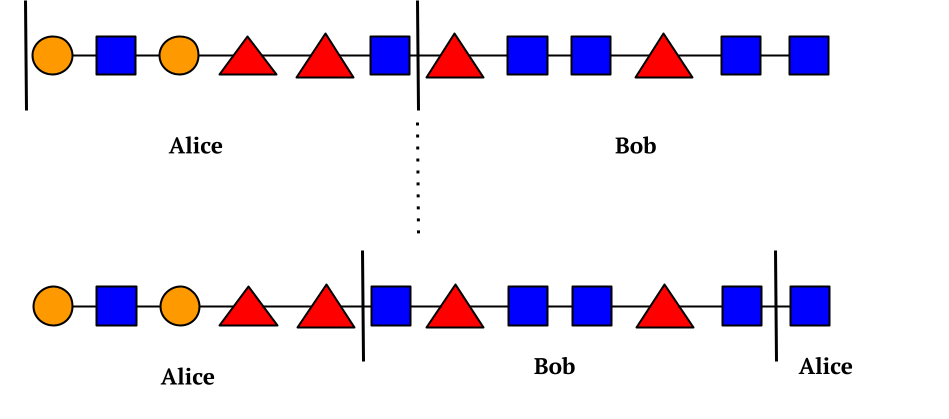
\includegraphics[scale=.35]{k=3.png}
\caption{n = 12, k = 3}
\label{4}
\end{figure}

Now we will follow the same methodology by shifting the cuts per one each time as the previous question. After that we will enumerate all the possibilities and arrange the results in a table \ref{tab:my-table}. We will use the following notation, for both Alice and Bob we will have (n1, n2, n3) such that n1, n2, n3 represent the number of rubies, diamonds, sapphires respectively. Note that in the fairness division we should have \textbf{(2, 3, 1)} for both of them.


\begin{table}[H]
\centering
\begin{tabular}{@{}
>{\columncolor[HTML]{FFFFFF}}l 
>{\columncolor[HTML]{FFFFFF}}l 
>{\columncolor[HTML]{FFFFFF}}l @{}}
\toprule
\multicolumn{1}{c}{\cellcolor[HTML]{FFFFFF}} & \multicolumn{1}{c}{\cellcolor[HTML]{FFFFFF}\textbf{Alice}} & \multicolumn{1}{c}{\cellcolor[HTML]{FFFFFF}\textbf{Bob}} \\ \midrule
\textbf{Initial cut}                          & (2, 2, 2)                                                  & (2, 4, 0)                                                \\
\textbf{1st shift}                           & (1, 4, 1)                                                  & (3, 2, 1)                                                \\
\textbf{2nd shift}                           & (1, 4, 1)                                                  & (3, 2, 1)                                                \\
\textbf{3rd shift}                           & (1, 3, 2)                                                  & (3, 3, 0)                                                \\
\textbf{4th shift}                           & (1, 3, 2)                                                  & (3, 3, 0)                                                \\
\textbf{5th shift}                           & (2, 2, 2)                                                  & (3, 3, 0)                                                \\
\textbf{6th shift}                           & (2, 2, 2)                                                  & (2, 4, 0)                                                \\ \bottomrule
\end{tabular}
\caption{Possibilities enumeration}
\label{tab:my-table}
\end{table}
We can noticed that after enumerating all the possibilities we did not mange to cut the necklace fairly between Alice and Bob using only 2-cut,


\section{Partition strategy}
In this part we will assume that $n_1$, $n_2$ and $n_3$ are even. Both Alice and Bob should receive exactly half of $n_i$. We will use the following strategy to repeat the division between Alice and Bob.

\begin{enumerate}

    \item start from the left, cut the necklace at the first position before reaching $\frac{n_i}{2}$ + 1.
    \item give it to the Alice.
    \item repeat step$_1$, but give it to Bob.
    \item repeat.
    
    
    
    
\end{enumerate}

We implemented the algorithm on our previous examples. As illustrated in figures \ref{5}, \ref{6}. We observed that we need 2 and 3 cuts with k = 2, k = 3 respectively, in order to reach the fair division between Alice and Bob.

\begin{figure}[H]
  \centering
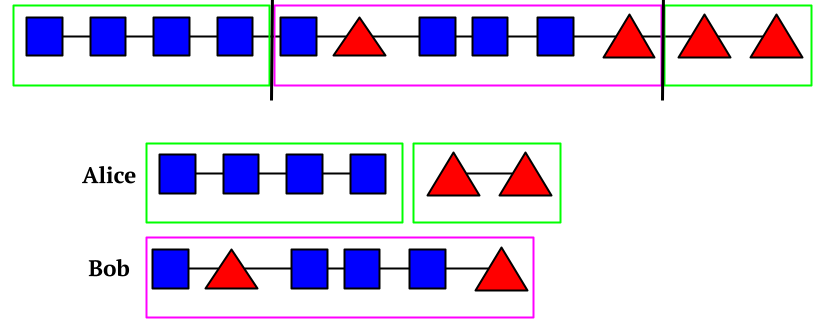
\includegraphics[scale=.4]{partition_strategy_k=2 (1).png}
\caption{Partition strategy, k = 2, cuts = 2}
\label{5}
\end{figure}

\begin{figure}[H]
  \centering
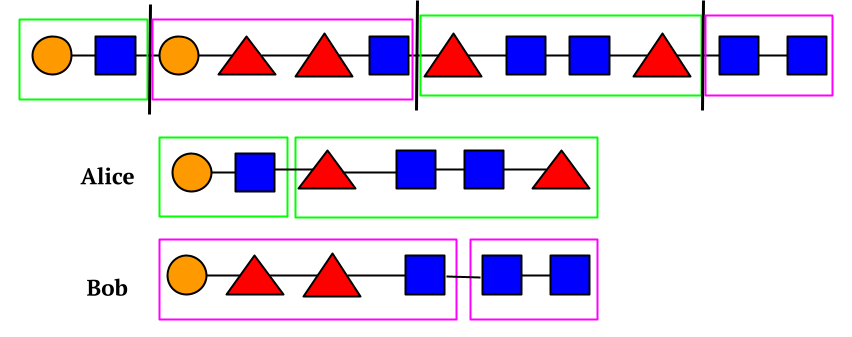
\includegraphics[scale=.35]{k = 3, cuts = 3.png}
\caption{Partition strategy, k = 3, cuts = 3}
\label{6}
\end{figure}

According to the initial necklace arrangement configuration. We might have a case where only one cut is sufficient. In this case we could divide the necklace on the middle and have the number of each jewels types distributed fairly between Alice and Bob ( the two intervals after cutting the necklace), as shown in the figure below \ref{7}:


\begin{figure}[H]
  \centering
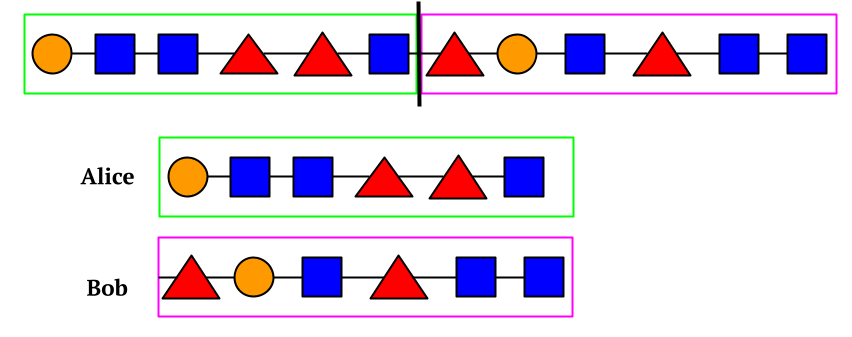
\includegraphics[scale=.35]{k= 3, cuts = 1.png}
\caption{Partition strategy, k = 3, cuts = 1}
\label{7}
\end{figure}


\section{Pseudo code}
In the algorithm below, we formalized the partition strategy in pseudo-code :

\begin{algorithm}[H]
\caption{Partition strategy}
\begin{algorithmic} [1]
\State $turn\gets0$
\State $C_1\gets[0,0,0]$
\State $C_2\gets[0,0,0]$
\While {$i \in necklace$} \Comment{to iterate over the necklace }
\If{$C_t_u_r_n[type(i)] = number_t_y_p_e_(_i_) \backslash 2$} \Comment{cutting condition }
    \State $turn = !turn$ \Comment{switch to another jewel type}
    \State $C_t_u_r_n[type(i)]++$
    \State $C\gets C \cup {\{i\}}$ \Comment{cut at this position}
 \Else 
 \State $C_t_u_r_n[type(i)]++$ \Comment{go to next jewel}
 \EndIf
\end{algorithmic}
\end{algorithm}

\section{More than three cuts}
We observed that by using our partition algorithm the number of cuts depends on the necklace jewels arrangement. In the previous example, 3 cuts are enough with 3 types of jewels. Now we will propose a different example to show that 3 cuts are not always enough to divide the necklace fairly between Alice and Bob, as shown in figure \ref{8}

\begin{figure}[H]
  \centering
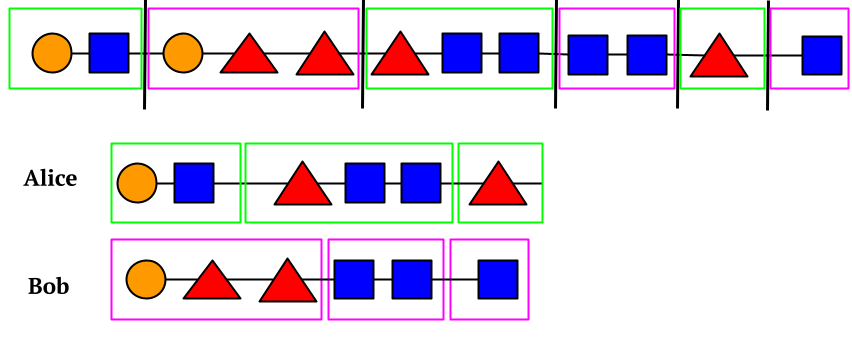
\includegraphics[scale=.38]{k = 3, cuts = 5.png}
\caption{Partition strategy, k = 3, cuts = 5}
\label{8}
\end{figure}
We noticed that we need 5 cuts in order to divide the necklace. The idea here is that we force the algorithm to do as much cut as possible by playing with jewels order.
% For instance, if we denote the necklace as list of size n
% $[0, 1, 2, ........ n_-_1, n]$




\section{Lower bound number of cuts}
Here in this part we tried to generalize our example with k = 3 by supposing that we have n1, n2, n3 number of jewels for each three types. In addition to that we have each type appears as a contiguous interval as shown in the figure below \ref{9}:

\begin{figure}[H]
  \centering
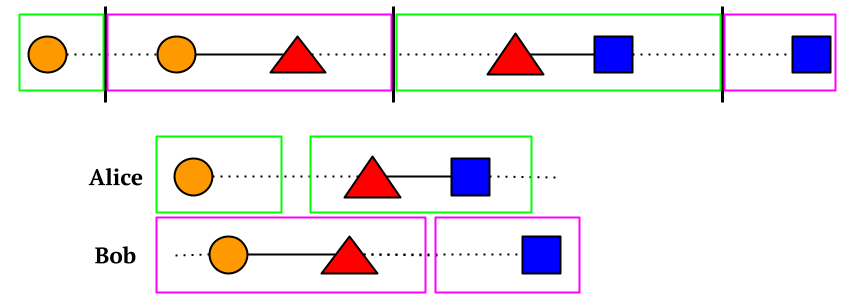
\includegraphics[scale=.38]{generalize_Partition_Strategy.png}
\caption{Lower bound, k = 3}
\label{9}
\end{figure}
We can observed that doing the division is possible with only three cuts. We need exactly one cut in the middle of each interval for each type. Using the same example, if we tried to cut each interval in the middle as shown in the figure above \ref{19}. We will have the sapphires of Alice on the leftmost interval of the necklace, then we will have the sapphires and rubies of Bob as a contiguous interval, the next interval will be the rubies and diamonds of Alice, finally we will have the the diamonds of Bob. As a result, if we have 2 thieves with k jewels types and each type appears as a contiguous interval in the necklace. It is always possible to cut the necklace with exactly k cuts. 
In addition to that, we can extend the example by increasing k (the number of jewels types). If we have a necklace composed of k types of jewels and each type appears as a contiguous interval in the necklace., it is always possible to divide it fairly between two thieves using k cuts. 


\section{Our strategy}
We can consider the following strategy to solve the problem. For a necklace composed of 3 types of jewels, we can denote the problem as follow:

\begin{itemize}
    \item $n$ : the total number of jewels in the necklace, $n = n_1 + n_2 + n_3$
    \item $n_i$, the number of each jewel of type $i$
\end{itemize}
We can describe our algorithm as follow:

\begin{enumerate}

    \item start from the first jewel on the left, depending on its type, check the whole necklace until you find an interval which satisfy the property $(\frac{n_i}{2} - 1, \frac{n_i}{2}, \frac{n_i}{2})$, cut the necklace.
    \item move to the second jewel.
    \item repeat $step_1$


\end{enumerate}
The main idea of our algorithm is that cutting the necklace at the beginning is less costly since we need only one cut to have a separated interval. After that, trying to find the interval which complete the first one. For instance: in figure\ref{11}, the first cut was after the first \textbf{sapphire}, we will search through out the necklace for a contiguous interval that exactly contained \textbf{(2 rubies, 3 diamonds)}. We will run the algorithm step by step with all examples presented in this report in order to illustrate the method and to determine the number of needed cuts.

\begin{figure}[H]
  \centering
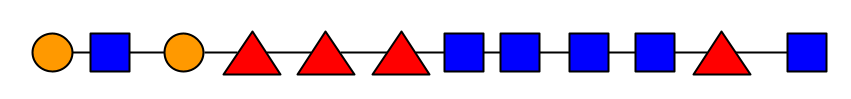
\includegraphics[scale=.4]{0_step (1).png}
\caption{Our example}
\label{10}
\end{figure}
Considering the above example , figure\ref{10}. We can notice that for the fairness division we should have \textbf{(2 rubies, 3 diamonds, 1 sapphire)} for both of Alice and Bob. Starting from the first sapphire we observed that we could find a contiguous interval that composed of \textbf{(2 rubies, 3 diamonds, 0 sapphire)}. Thus, we split the necklace exactly after the first sapphire and isolated the desired interval with two cuts (one cut before the first jewel and one cut after the last jewel). The proportion for the second thief would be fixed as well. Our problem can be solved with exactly 3 cuts, as shown in the figure below \ref{11}:


\begin{figure}[H]
  \centering
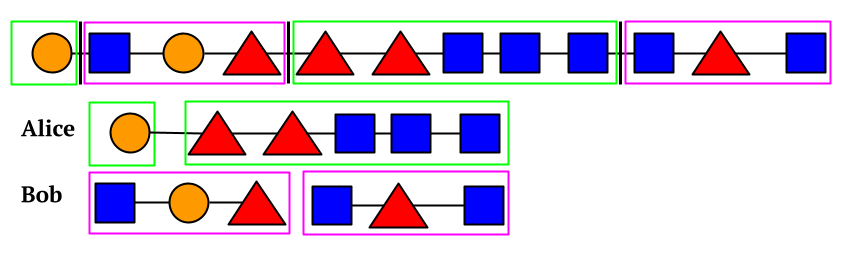
\includegraphics[scale=.4]{first_step (2).png}
\caption{Necklace after division using our algorithm}
\label{11}
\end{figure}

As a result, in our algorithm we only need 3 cuts to divide the necklace between Alice and Bob, comparing to 5 cuts if we used the given algorithm.

\subsection{More sophisticated example}
Now we will implement our algorithm on a more complicated example, as shown in the figure below, the necklace is composed of 22 jewels (10 rubies, 8 diamonds, 4 sapphire). Therefor, each Alice and Bob should have an interval with exactly \textbf{(5 rubies, 4 diamonds, 2 sapphire)} at the end of division, as shown in the figure \ref{12}

\begin{figure}[H]
  \centering
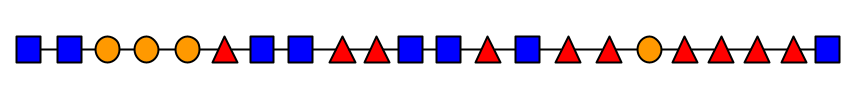
\includegraphics[scale=.42]{sophistacated.png}
\caption{More sophisticated example}
\label{12}
\end{figure}

We noticed that after the third jewel ( the first sapphire ), we could exactly have a contiguous interval with exactly  \textbf{(5 rubies, 2 diamonds, 1 sapphire)}. We cut the necklace after the third jewel and isolated the desired interval using 2 cuts. As a result, we will have a fair division of the necklace with exactly 3 cuts, as  as illustrated in the figure below \ref{13}.

\begin{figure}[H]
  \centering
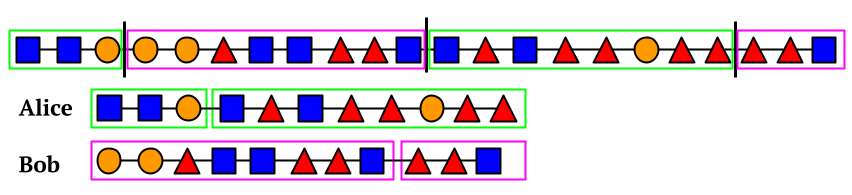
\includegraphics[scale=.42]{sophistacated_cuted.png}
\caption{Fair division of the necklace with exactly 3 cuts}
\label{13}
\end{figure}

Now we will solve the same example using the given partition algorithm, in order to compare between solutions, as shown in figure \ref{14}
\begin{figure}[H]
  \centering
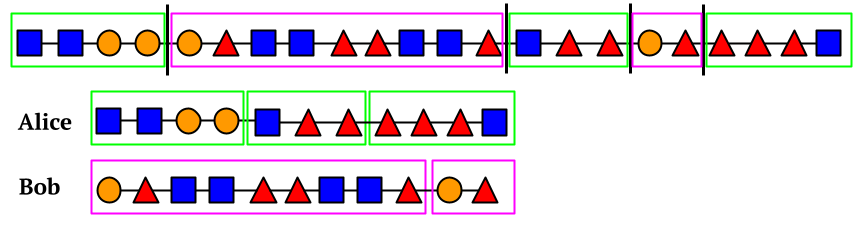
\includegraphics[scale=.42]{sophisticated_using_partition.png}
\caption{Fair division of the necklace with exactly 4 cuts}
\label{14}
\end{figure}

As a result, we need 3 cuts to divide the necklace using our algorithm. On the other hand, if we used the given partition algorithm, we need 4 cuts.




\section{Special case of necklace with k pairs of jewels}
\subsection{Preliminary examples  }
In this section, we assume that the necklace composed of of k types, where the number of jewels for each is equal to 2. We will try to find the optimal solution. First of all, we will introduce a counter example and figure out different configurations of necklace jewels arrangement, in order to reach the optimal algorithm. In the following example we have 12 jewels ( 6 different types ) as shown in the figure below \ref{15}. We can divide the necklace fairly between Alice and Bob with exactly one cut since we have exactly one jewel of each types in the both half of the necklace as illustrated below, figure \ref{15}.

\begin{figure}[H]
  \centering
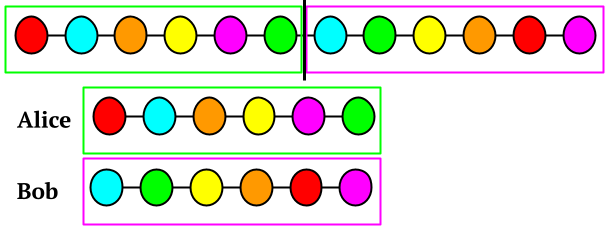
\includegraphics[scale=.45]{k=6, cuts = 1.png}
\caption{k = 6 , cuts = 1}
\label{15}
\end{figure}

In the following example figure \ref{16}, we noticed that we should have 2 cuts at least in order to divide the necklace fairly between Alice and Bob. Actually, the number of cuts depends on the different initial configurations of the necklace jewels.

\begin{figure}[H]
  \centering
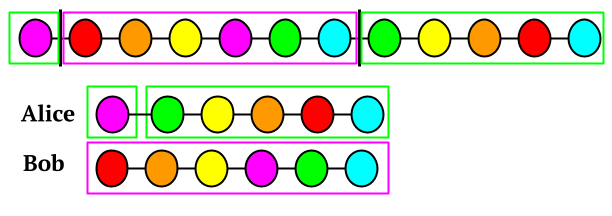
\includegraphics[scale=.50]{_k=6 , two cut.png}
\caption{k = 6 , cuts = 2}
\label{16}
\end{figure}

In the next two sections, we will propose a general algorithm for dividing the necklace. We will consider two main cases, the first one is when the necklace is composed of an odd numbers of jewels pairs, while the second one is when the necklace is composed of an even number of jewels pairs. We will discuss the two cases and analyze the optimal solution.
\subsection{Odd number of pairs}
We have an odd odd number of pairs. Our purpose is to have the worst case configuration of the necklace, where each pair appears consecutively, as shown in the following example, figure\ref{17}.
\begin{figure}[H]
  \centering
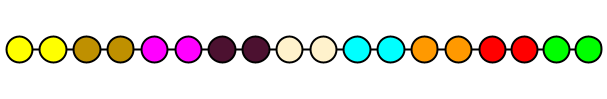
\includegraphics[scale=.60]{k is odd (1).png}
\caption{Number of pairs, k = 9}
\label{17}
\end{figure}

If we have an odd number of pairs, we will have the same division pattern as shown in figure \ref{18}.
\begin{figure}[H]
  \centering
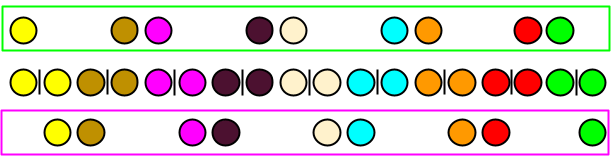
\includegraphics[scale=.60]{k is odd after division.png}
\caption{k = 9, cuts = 9}
\label{18}
\end{figure}


\newpage\subsection{Even number of pairs}
Here we have an even number of pairs. As we did previously, we will construct the scenario, where each pair appears consecutively, as shown in the following example, figure\ref{19}.
\begin{figure}[H]
  \centering
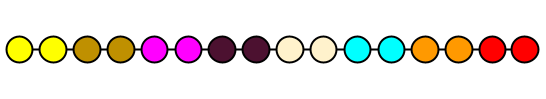
\includegraphics[scale=.55]{k is even.png}
\caption{Number of pairs, k = 8}
\label{19}
\end{figure}

If we have an odd number of pairs, we will have the same division pattern as shown in figure \ref{20}.
\begin{figure}[H]
  \centering
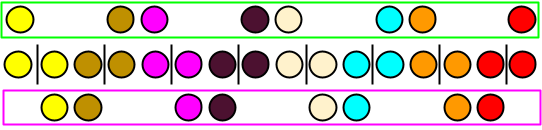
\includegraphics[scale=.55]{k is even after division.png}
\caption{k = 8, cuts = 8}
\label{20}
\end{figure}
\subsection{Conclusion}
According to our previous examples, we can observe that it is always possible to do the division with at most \texttt{K} cuts, where k is the number of pairs composed the necklace.






\begin{thebibliography}{9}
\bibitem{article}
Alon, N. and Graur, A., 2020. Efficient splitting of measures and necklaces. arXiv preprint arXiv:2006.16613.

\end{thebibliography}




\end{document}